\chapter{Espacios vectoriales}

\hlpink{TODO: usar notación de span para subespacios. No quiero que
se confunda eso con el producto punto.}


¿Qué entiendes por un \textit{vector}?

En clases previas de física, usabas estos objetos para representar
\textit{fuerzas} pues, para hablar de una fuerza,
se necesita especificar tanto su 
\textit{magnitud} como su 
\textit{dirección}.
\marginnote{Por ejemplo, la fuerza de gravedad que ejerce el planeta Tierra
en los objetos sobre ella es de $9.8 m/s^{2}$, pero ¿qué dirección tiene?}


Algunos aspectos implícitos eran que 
\begin{itemize}
\item los vectores eran elementos de
$\IR^{2}$ o de $\IR^{3}$, 
\item podías ``sumar vectores'' usando la ley
del paralelogramo (por ejemplo, si varias fuerzas actuan en un objeto, las sumabas para
obtener la \textit{fuerza neta} ejercida en el objeto),
\item además, podías ``multiplicar vectores
por números reales'' para cambiar su 
magnitud y, dependiendo del signo del número real,
mantener la dirección o invertirla (considera, por ejemplo, la 
segunda Ley de Newton: $\hat{F} = m \hat{a}$).
\end{itemize}

\begin{center}
\begin{figure}[H]
	\centering
	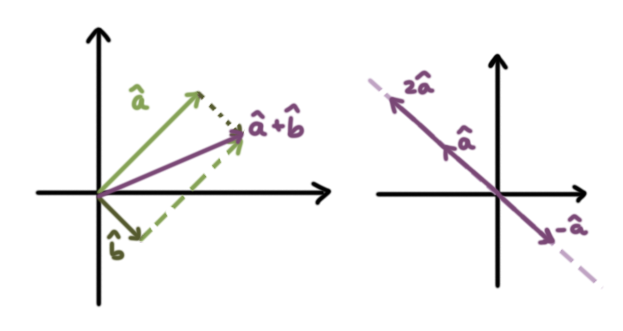
\includegraphics[scale= 3.2]{28} 
\end{figure}
\end{center}


Estas manipulaciones geométricas además satisfacen
ciertas propiedades algebráicas; por ejemplo, 
dados tres vectores $\hat{a}, \hat{b}, \hat{c} \in \IR^{2}$
y dos escalares $m, n \in \IR$, puedes comprobar geométricamente que
\[
\hat{a} + (\hat{b} + \hat{c}) = (\hat{a} + \hat{b}) + \hat{c},
\]
\begin{equation}
	\label{eq: 1}
	m (\hat{a} + \hat{b}) = m \hat{a} + m \hat{b},
\end{equation}
o que 
\[
m(n\hat{a}) = (mn) \hat{a}.
\]

Abstrayendo este escenario, tenemos
\begin{itemize}
	\item un conjunto $V$ de ``vectores'', que pueden ser sumados entre sí,
	\item otro conjunto $F$ de ``escalares'', cuyos elementos pueden multiplicarse 
	por elementos de $V$. En $F$ además se pueden hacer sumas y productos.
	\item Además, tenemos ciertas relaciones entre las operaciones de $F$ y $V$
	(c.f. \eqref{eq: 1}).
\end{itemize}

\section{Algunas estructuras algebráicas}
Ya comentamos antes que sabíamos sumar vectores en el plano o 
en el espacio; empecemos pues por abstraer el 
concepto de operación. Estamos acostumbrados a sumar 
números reales: dados $a, b \in \IR$, conocemos una
\textit{regla} para asignarle a la pareja $(a, b)$
un número real llamado su suma, que solemos denotar por $a+b$.
También hablamos de la resta de los números $a, b$.
Observe que estas operaciones tienen distintas propiedades, por
ejemplo, la suma es asociativa y conmutativa, pero
la resta no. 
\begin{defi}
Dado $X \neq \emptyset$ un conjunto no vacío, una
\textbf{operación binaria} en $X$ es una función con dominio
$X \times X$ y codominio $X$.
\end{defi}
O sea, una operación binaria $*: X \times X \longrightarrow X$ 
es una regla que a cada para ordenado $(x_{1}, x_{2})$ le asigna
un único elemento $x_{3}$ de $X$. Por ser este elemento único,
puede dársele un nombre; es usual denotar a $x_{3}$
por $x_{1} * x_{2}$.
\marginnote{Es decir, con $x_{1} * x_{2}$ estamos abreviando a 
$*(x_{1}, x_{2})$.}

\begin{defi}
Dado $X \neq \emptyset$ y $+: X \times X \longrightarrow X$
una operación binaria en $X$, la pareja $(X, +)$ es un \textbf{grupo}
si 
\begin{itemize}
	\item[GR-1)] \textit{(asociatividad)} Para cualesquiera 
	$x_{1}, x_{2}, x_{3} \in X$,
	\marginnote{La asociatividad de la operación $*$
	significa en la práctica que los paréntesis en 
	\eqref{eq: grupo asociatividad} pueden omitirse.}
	\begin{equation}
		\label{eq: grupo asociatividad}
		(x_{1} + x_{2} ) + x_{3} = x_{1} + (x_{2} + x_{3}).
	\end{equation}
	\item[GR-2)] \textit{(existencia de elemento neutro)} Existe
	$e \in X$ tal que 
	\begin{equation}
		\label{eq: grupo e}
		\forall x \in X: \hspace{0.2cm}
		e + x = x = x + e.
	\end{equation}
	\item[GR-3)] \textit{(existencia de inversos)} 
	Se cumple que 
	\begin{equation}
		\label{eq: grupo inversos}
		\forall x \in X \hspace{0.1cm}
		\exists -x \in X: \hspace{0.2cm}
		x + (-x) = e = (-x) + x.
	\end{equation}
\end{itemize}
\end{defi}
Es fácil demostrar la unicidad del elemento neutro y de los inversos
- por eso es legítimo darles un nombre particular a estos en la 
definición de grupo.
Si la operación binaria $+$ se entiende por el contexto, al grupo
$(X, +)$ se le denota por $X$.
\begin{defi}
A todo grupo $(X, +)$ que satisfaga que 
\begin{itemize}
	\item[GR-4)] \textit{(conmutatividad)}
	\begin{equation}
		\label{eq: grupo conmut}
		\forall x_{1}, x_{2} \in X : \hspace{0.2cm}
		x_{1} + x_{2} = x_{2} + x_{1}
	\end{equation}
	se le llamará \textbf{abeliano}.
\end{itemize}
\end{defi}


La motivación del concepto de grupo es tener un conjunto con una
operación binaria en el que se puedan hacer cancelaciones;
si en un grupo $(G, +)$ se tiene una ecuación de la forma
\[
a + b = a + c,
\]
sumando a ambos lados de la igualdad el inverso de $a$ 
y usando el que la operación sea asociativa, se tiene que 
\[
e + b = e + c,
\]
luego, que 
\[
b = c.
\]

\begin{ejem}
Considera al conjunto $\IZ$ de los números enteros.
\begin{itemize}
	\item Si $+$ denota a la suma usual de números enteros,
	comprueba que $(\IZ, +)$ es un grupo.
	\marginnote{Este último punto muestra que frases del tipo
	``el conjunto $X$ es un grupo'' son ambiguas. Puede ser posible
	definir dos operaciones binarias $+$ y $\cdot$ en $X$
	de tal forma que tanto $(X, +)$ como $(X, \cdot)$ sean
	grupos. Los conjuntos subyacentes de estos grupos son los mismos,
	pero estos no son el mismo grupo.}
	\item Muestra que, si $\cdot$ denota al producto usual 
	de enteros, $(\IZ, \cdot)$ \textit{no} es un grupo.
	\item Si ahora $+$ y $\cdot$ denotan, respectivamente, la
	suma y producto de números racionales, demuestra que
	tanto $(\IQ, +)$ como $(\IQ - \{ 0 \}, \cdot)$ son grupos abelianos.
\end{itemize}
\end{ejem}


\begin{defi}
Dado $F \neq \emptyset$ un conjunto no vacío y dos operaciones binarias
$+ : F \times F \longrightarrow F$ y $\cdot: F \times F \longrightarrow F$,
$(F, +, 0, \cdot, 1)$ con $0 \neq 1$ es un \textbf{campo} si 
\begin{itemize}
	\item $(F, +)$ es un grupo abeliano con neutro $0$, es decir, si 
	\begin{itemize}
		\item $\forall a, b, c \in F$: $a + (b + c) = (a + b) + c$,
		\item $\forall a \in F$: $a + 0 = a = 0 + a$,
		\item $(\forall a \in F)$ $(\exists -a \in X)$: $a + (-a) = 0 = (-a) + a$,
		\item $\forall a, b \in F$: $a + b = b + a$,
	\end{itemize}
	\item $(F- \{ 0 \}, \cdot)$ es un grupo abeliano con neutro $1$, es decir,
	\begin{itemize}
		\item $\forall a, b, c \in F-\{0\}$: $a \cdot (b \cdot c) = (a \cdot b) \cdot c$
		\item $\forall a \in F - \{0\}:$ $a \cdot 1 = a = 1 \cdot a$,
		\item $(\forall a \in F - \{0\})$ $(\exists a^{-1} \in F- \{0\})$:
		$a \cdot a^{-1} = 1 = a^{-1} \cdot a$,
		\item $\forall a, b \in F - \{0\}$: $a \cdot b = b \cdot a$.
	\end{itemize}
	\item \textit{(distributividad)} 
	Para cualesquiera $a, b, c \in F$:
	\begin{equation}
		\label{eq: campo distrib}
		a \cdot (b + c) = a \cdot b + a \cdot c.
	\end{equation}
\end{itemize} 
\end{defi}
La distributividad es la propiedad que relaciona las estructuras
$(X, +)$ y $(X, \cdot)$ que conforman un campo. Por costumbre,
al neutro de $(X, +)$ se le suele llamar el \textbf{neutro aditivo}
del campo, y al neutro de $(X-\{ 0 \}, \cdot)$ se le llama el
\textbf{neutro multiplicativo}.

Por tener la ley distributiva, si $x \in X$ cualquiera,
\[
x \cdot 0 = x \cdot (0 + 0) = x \cdot 0 + x \cdot 0,
\]
luego, 
\[
x \cdot 0 = 0.
\]
Así, no existe $x \in X$ tal que $x \cdot 0 = 1$; por eso 
se debe quitar el cero para hablar del grupo multiplicativo
$(X- \{ 0 \}, \cdot)$.

\section{Definición de espacio vectorial}
Ya tenemos los elementos necesarios para dar una de las definiciones
centrales del curso.

\begin{defi}
	\label{defi: espacio vectorial}
	Sean $(V, +)$ un grupo abeliano y $F$ un campo. Si 
	$\cdot : F \times V \longrightarrow V$ es tal que 
	\marginnote{La función $\cdot$ (que no es una operación binaria, ¿verdad?)
	es la que conecta las estructuras de grupo abeliano y de campo que conforman
	a un espacio vectorial.}
	\begin{itemize}
		\item[EV-5)] $(\forall x \in V):$ $1_{F} \cdot x = x$,
		\item[EV-6)] $(\forall a, b \in F) (\forall x \in V):$
		$(ab) \cdot x = a \cdot (b \cdot x)$,
		\item[EV-7)] $(\forall a \in F)(\forall x, y \in V):$
		$a\cdot (x + y) = a \cdot x + a \cdot y$,
		\item[EV-8)] $(\forall a, b \in F)(\forall x \in V): $
		$(a+b) \cdot x = a \cdot x + b \cdot x $,
	\end{itemize}
	entonces $(V, + F, \cdot)$ es un \textbf{$F$-espacio vectorial}.
\end{defi}
Recuerda que, el que $(V, +)$ sea grupo abeliano, significa que 
\begin{itemize}
	\item[EV-1)] $(\forall x, y, z V):$ $x + (y+z) = (x+y) + z$,
	\item[EV-2)] $(\exists 0_{V} \in V) (\forall x \in V):$
	$0_{V} + x = x = x + 0_{V}$,
	\item[EV-3)] $(\forall x \in V)(\exists -x \in V):$
	$x + (-x) = 0_{V} = (-x) + x$,
	\item[EV-4)] $(\forall x, y \in V): $
	$x+y = y +x$.
\end{itemize}

Por tradición, a los elementos de $V$ se les llama ``vectores'' y a los
de $F$ ``escalares''. Nota que los vectores entonces son los elementos del 
grupo abeliano (cuyos elementos no necesariamente pertenecen a $\IR^{2}$
o $\IR^{3}$).

Se permite en la definición de espacio vectorial que $F$ sea cualquier campo
pero, a menos que se indique lo contrario, en lo que sigue entenderemos que
$F \in \{ \IR, \IC \}$.
Si hay riesgo de confusión, al vector cero se le denotará por $\hat{0}$
y al escalar cero se le denota por $0_{F}$. 


\section{Ejemplos de espacios vectoriales}
Vamos a dar las construcciones de espacios vectoriales concretos con los 
que trabaremos ampliamente en el curso.
En la lista de ejercicios \ref{section: ejercicios I}
se dan más ejemplos.

\subsection{El $F-$espacio vectorial $F^{n}$}
Sea $n \geq 1$ entero.
Tanto $\IR^{n}$ como $\IC^{n}$ con la suma definida ``entrada a entrada''
son grupos abelianos:

\begin{equation}
	\label{eq: suma en Rn}
	\forall x = (x_{k})_{k=1}^{n}, y = (y_{k})_{k=1}^{n} \in \IR^{n}:
	\hspace{0.2cm} x + y := (x_{k} + y_{k})_{k=1}^{n}.
\end{equation}
De forma similar, fijado un campo, podemos definir multiplicación 
escalar ``entrada a entrada'': si 
$\cdot : \IR \times \IR^{n} \longrightarrow \IR^{n}$ se define como 
\begin{equation}
	\label{eq: mult escalar en Rn}
	\forall x = (x_{k})_{k=1}^{n} \in \IR^{n}, a \in \IR:
	\hspace{0.2cm} ax := (ax_{k})_{k=1}^{n},
\end{equation}
puede comprobarse que $\IR^{n}$ con esta multiplicación escalar es un
$\IR-$espacio vectorial.
De forma similar se puede definir una $\IC-$multiplicación escalar en 
$\IC^{n}$ y también una $\IR-$multiplicación escalar en $\IC$.
¿Por qué no tiene sentido cambiar al campo de escalares en \eqref{eq: mult escalar en Rn}
por $\IC$?


En general, si $F$ es un campo y se considera el grupo abeliano
$F^{n}$ de $n-$tuplas con entradas en $F$ y suma definida como en 
\eqref{eq: suma en Rn}, con la multiplicación 
escalar definida como en \eqref{eq: mult escalar en Rn}, obtenemos un 
$F-$espacio vectorial. Haciendo $n = 1$, se tiene que $F$ es también un 
$F-$espacio vectorial (la multiplicación por escalares en este contexto es
la multiplicación en el campo $F$).

\begin{ejem}
	El grupo abeliano $\IR^{n}$ con la suma entrada a entrada con la multiplicación
	por escalares entrada a entrada es un $\IR-$espacio vectorial.
	$\IC^{n}$ puede ser visto como $\IC-$espacio vectorial o como $\IR-$espacio vectorial,
	dependiendo de en qué campo se tomen los escalares.
\end{ejem}

\subsection{El $F-$espacio vectorial $F^{X}$ de funciones de $X$ en $F$}
\label{subs: F ev de funciones de X en F}
Vamos ahora a definir espacios vectoriales cuyos vectores son funciones;
lo hacemos de esta forma porque esta construcción general engloba varios
ejemplos de interés práctico, por ejemplo, a los espacios de sucesiones o espacios
de funciones continuas - ambos importantes en el análisis - o el
espacio de polinomios con coeficientes en un campo.

Sean $X \neq \emptyset$ un conjunto no vacío cualquiera
y $(F, +, 0, \cdot, 1)$ un campo. Consideremos al conjunto
\[
F^{X} := \{ f: X \longrightarrow F :
\hspace{0.2cm} f \textit{ es función} \} 
\]
de funciones de $X$ en $F$; aprovechando la estructura de campo
en $F$, vamos a dotar al conjunto $F^{X}$ de estructura
de $F-$espacio vectorial.\\

\begin{itemize}
	\item \textbf{Definición de suma de funciones:}
	Definimos a la operación binaria suma
	\begin{equation}
		\label{eq: suma de funciones}
		\hat{+} : F^{X} \times F^{X} \longrightarrow F^{X}
	\end{equation}
	como sigue: dadas $f, g \in F^{X}$ cualesquiera, 
	la función $f \hat{+} g \in F^{X}$ se define puntualmente como
	\begin{equation}
		\label{eq: suma funciones puntual}
	(f \hat{+} g)(x) = f(x) + g (x), \hspace{0.2cm}
	x \in X.
	\end{equation}
	Nota que, en la ecuación anterior, el signo $\hat{+}$
	que aparece a la izquierda es la operación binaria
	que estamos definiendo en \eqref{eq: suma de funciones}, 
	mientras que el signo $+$ de la derecha es la suma
	del campo $F$: \textit{a partir de la operación
	suma en $F$ estamos diciendo cómo sumar elementos
	de $F^{X}$}.
	
	\item \textbf{Definición de producto por escalares:}
	Definimos a un producto por escalares
	\begin{equation}
		\label{eq: producto por escalares}
	\star : F \times F^{X} \longrightarrow F^{X} 	
	\end{equation}		
	como sigue: si $a \in F$ y $f \in F^{X}$, la función
	$a \star f \in F^{X}$ se define puntualmente como
	\begin{equation}
		\label{eq: definicion prod esc}
	(a \star f)(x) = a f(x), \hspace{0.2cm}
	x \in X.
	\end{equation}
	Nota cómo estamos usando la operación producto
	del campo para definir el producto por escalares.
	
	\item \textbf{Neutro aditivo:} Proponemos como 
	neutro para la operación suma de funciones (c.f. \eqref{eq: suma de funciones}) a la función $\hat{0} : X \longrightarrow F$
	definida como sigue:
	\begin{equation}
		\label{eq: funcion cero}
		\hat{0}(x) = 0, \hspace{0.2cm} x \in X,
	\end{equation}
	es decir, a la función que mapea todo punto
	de $X$ al neutro aditivo del campo $F$.
\end{itemize}

Demostremos que 
$(F^{X}, \hat{+}, \star)$
es un $F-$espacio vectorial.\\


En lo que sigue, vamos a demostrar igualdades que tienen lugar
en $F^{X}$, es decir, igualdades entre funciones.
Recuerda que dos funciones son iguales si tienen el mismo dominio,
codominio y misma regla de correspondencia: puesto que todos los 
elementos de $F^{X}$ tienen dominio $X$ y codominio $F$, para
demostrar que $f, g \in F^{X}$ son iguales basta ver que
\[
f(x) = g (x) \hspace{0.2cm}
\textit{ para toda } x \in X.
\]

\begin{enumerate}
	\item \textbf{Asociatividad de $\hat{+}$:}
	sean $f, g, h \in F^{X}$. Mostremos que 
	\[
	(f \hat{+} g) \hat{+} h = f \hat{+} ( g \hat{+} h).
	\]
	Sea $x \in X$.
	Usando la definición de suma de funciones dada en 
	\eqref{eq: suma funciones puntual},
	tenemos que 
	\begin{align*}
	((f \hat{+} g) \hat{+} h )(x) = &
	(f \hat{+} g)(x) + h(x)
	= (f(x) + g(x)) + h(x) \\
	= & f(x) + (g(x) + h(x)) = f(x) + (g \hat{+} h)(x) \\
	= & (f \hat{+} (g \hat{+} h)) (x).
	\end{align*}
	La tercera igualdad se da porque la suma en $F$
	es asociativa.
	
	\item \textbf{Elemento neutro para la suma:}
	Si $f \in F^{X}$ cualquiera, veamos que
	\[
	\hat{0} \hat{+} f = f = f \hat{+} \hat{0}.
	\]
	Probemos la primera igualdad; la otra se tiene de forma 
	análoga. Usaremos la definición 
	\eqref{eq: funcion cero}
	de la función cero $\hat{0}$ y la definición de suma de funciones dada en 
	\eqref{eq: suma funciones puntual}.
	Para toda $x \in X$,
	\[
	(\hat{0} \hat{+} f) (x) = 
	\hat{0}(x) + f(x) = 0 + f(x) = f(x).
	\]
	
	\item \textbf{Existencia de inversos aditivos:}
	\hlgray{Ejercicio:} Dada una función $f \in F^{X}$, propón
	una función $g \in F^{X}$ que sea el neutro
	aditivo de $f$, es decir, una función tal que
	\[
	f \hat{+} g = \hat{0} = g \hat{+} f.
	\]
	Sugerencia: Defínela puntualmente, usa la existencia
	de inversos aditivos en el campo $F$.
	Naturalmente, a tal función $g$ la denotaremos por $-f$.
	
	\item \textbf{Conmutatividad de $\hat{+}$}:
	\hlgray{Ejercicio:} Demuestra que la suma de funciones
	es conmutativa, es decir, que dadas cualesquiera
	$f, g \in F^{X}$, 
	\[
	f \hat{+} g = g \hat{+} f.
	\]
	
	\item \textbf{(EV-5)} Sea $f \in F^{X}$ cualquiera;
	es fácil ver que ocurre
	\[
	1 \star f = f
	\]
	pues, según la definición del producto por escalares dada en 
	\eqref{eq: definicion prod esc}, 
	para toda $x \in X$ se tiene que
	\[
	(1 \star f)(x) = 1 f(x) = f(x).
	\]
	\item \textbf{(EV-6)} Si $a, b \in F$
	y $f \in F^{X}$, demostremos que
	\[
	(ab) \star f = a \star (b \star f).
	\] 
	Sea $x \in X$.
	\[
	((ab) \star f)(x) = ab f(x) = a (bf(x))
	= a ((b \star f)(x)) = (a \star (b \star (f)))(x).
	\]
	\item \textbf{(EV-7)}
	\hlgray{Ejercicio: } Demuestra que,
	para todo $a \in F$ y cualesquiera
	$f, g \in F^{X}$, 
	\[
	a \star (f \hat{+} g) = a \star f \hat{+} a \star g.
	\]
	
	\item \textbf{(EV-8)}
	\hlgray{Ejercicio: } Demuestra que,
	para toda $f \in F^{X}$ y cualesquiera
	$a, b \in F$, 
	\[
	(a + b) \star f = a \star f \hat{+} b \star f.
	\]
	
\end{enumerate}

\begin{ejem}
Si $\mathcal{C}(\IR) = \{ f: \IR \longrightarrow \IR :
\hspace{0.2cm} f \textit{ es continua} \}$,
es claro que 
$\mathcal{C}(\IR) \subseteq \IR^{\IR}$.
\end{ejem}


\subsection{Espacio de funciones de soporte finito $F^{(X)}$}

\begin{defi}
Sean $X \neq \emptyset$ un conjunto, $F$ un campo. Dada
$f: X \longrightarrow F$ función (i.e. un elemento
de $F^{X}$), definimos su \textbf{soporte}
\begin{marginfigure}
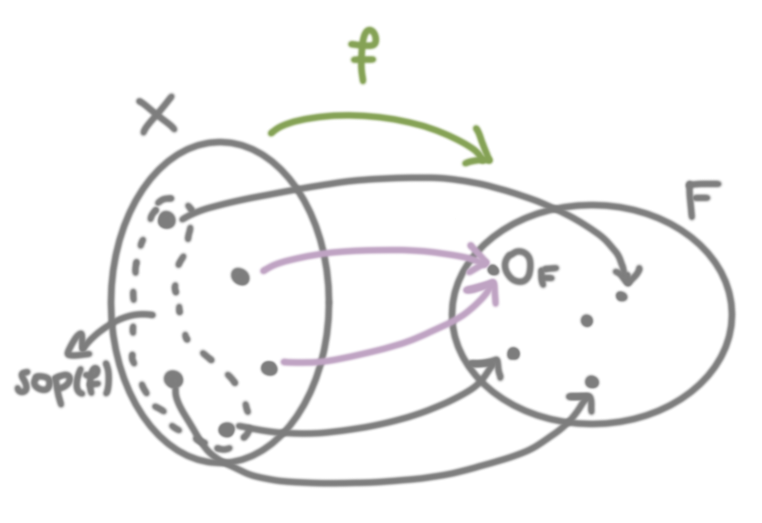
\includegraphics[scale= 1.3]{ 1} 
		\caption{Representación gráfica del soporte de una función.}
\end{marginfigure}
como el conjunto de los puntos del dominio para 
los que $f$ no se anula:
\[
sop(f) :=
\{ x \in X  | \hspace{0.2cm} f(x) \neq 0 \}.
\]

\end{defi}

\begin{ejem}
Tomemos a $X = \IN$. Acostumbramos llamar a los 
elementos de $F^{\IN}$ 
(i.e. a las funciones de $\IN$ en $F$)
\textbf{sucesiones en $F$}.
De hecho, dada una función $f \in F^{\IN}$, 
es usual identificarla con el conjunto de sus imágenes:
\[
f = (f_{n})_{n \in \IN}, 
\hspace{0.2cm} \textit{ donde }
f_{n} := f(n).
\]
\hlgray{Ejercicio:} Demuestre que,
si $f = (f_{n})_{n \in \IN} \in F ^{\IN}$ tiene soporte 
finito, entonces 
se debe tener
$\lim_{n \rightarrow \infty} f(n) = 0$.
¿Se vale la otra implicación?
\diam
\end{ejem}


\begin{defi}
Denotaremos por $F^{(X)}$ al conjunto de las funciones
de $X$ en $F$ que tienen soporte finito, es decir,
\[F^{(X)} := \{ f \in F^{X}  : \hspace{0.2cm}  
|sop(f) | < \infty \}.
\]
\end{defi}


Para lo que sigue, necesitamos que el lector recuerde
(o al menos esté de acuerdo en aceptar como ciertos)
los siguientes hechos:
\begin{itemize}
	\item La cardinalidad del conjunto vacío es $0$.
	El conjunto vacío es el único conjunto de cardinalidad $0$.
	\item Si $A$ y $B$ son dos conjuntos finitos, entonces
	$A \cup B$ es también finito.
	\item Si $A$ está contenido en $B$ y $B$ es finito, entonces
	$A$ también lo es.
\end{itemize}

\begin{prop}
Si $X \neq \emptyset$ y $F$ es un campo, entonces
$F^{(X)}$ es un subespacio de $F^{X}$.
\end{prop}
\noindent
\textbf{Demostración.}
Usemos los criterios dados en la proposición $(*-sub)$
para mostrar que $F^{(X)} \leq F^{X}$.
\begin{enumerate}
	\item Si $\hat{0}: X \longrightarrow F$ es la función
	cero, 
	\[
	sop(\hat{0}) = \{ x \in X  | \hspace{0.2cm} \hat{0}(x) \neq 0\}
	= \emptyset,
	\]
	luego, $\hat{0}$ tiene soporte finito, o sea, 
	$\hat{0} \in F^{(X)}$.
	
	\item Sean $f, g \in F^{(X)}$; veamos que $f + g \in F^{(X)}$.
	Es decir, usando que $f$ y $g$ tienen soporte finito, mostremos
	que $f+g$ también tiene soporte finito.
	Si $sop(f + g) = \emptyset$, acabamos. Supongamos ahora
	que $sop(f+g) \neq \emptyset$. Note que, si 
	$x \in sop(f+g)$, entonces
	\[
	f(x) + g(x) = (f+g)(x) \neq 0,
	\]	
	luego, no ocurre $f(x) = 0 = g(x)$, es decir,
	\[
	x \not\in (sop(f))^{c} \cap (sop(g))^{c},
	\]
	o sea, 
	\[
	x \in sop(f) \cup sop(g).
	\]
	Con esto demostramos la contención
	\[
	sop(f+g) \subseteq sop(f) \cup sop(g).
	\]
	Como $sop(f)$ y $sop(g)$ son, por hipótesis, ambos
	finitos, su unión también lo es, luego
	$sop(f+g)$, por ser subconjunto de un conjunto finito,
	es finito.
	
	\item Sean $f \in F^{(x)}$ y $a \in F$; probemos que
	$af \in F^{(X)}$. Si $a = 0$, 
	$a f = \hat{0} \in F^{(X)}$; supongamos ahora $a \neq 0$.
	\marginnote{Recuerda que, en un campo, el producto de dos
	elementos es cero si y sólo si al menos uno de los dos es cero.}
	Entonces,
	\begin{align*}
	x \in sop(af) & \Leftrightarrow  af(x) \neq 0 \\
	& \Leftrightarrow  a \neq 0 \textit{ y } f(x) \neq 0 \\
	& \Leftrightarrow  f(x) \neq 0 
	\Leftrightarrow x \in sop(f).
	\end{align*}
	Así, $sop(a f) = sop(f)$, luego, $af$ tiene, al igual
	que $f$, soporte finito.
\end{enumerate}

\QEDB
\vspace{0.2cm}

\begin{nota}
	Por un polinomio, por lo general se entiende una función
	$f: F \longrightarrow F$
	de la forma 
	\begin{equation}
		\label{eq: pol en x}
	f(x) = a_{0} + a_{1}x + \ldots + a_{n}x^{n}, \hspace{0.2cm}
	n \in \IN, a_{k} \in F,
	\end{equation}
	con los ``coeficientes'' $a_{k} \in F$ y la ``incógnita''
	$x$, que puede tomar valores en el campo $F$.
	\marginnote{En realidad, basta con partir de un anillo $R$ - que no necesariamente
	sea campo -  para construir al anillo de polinomios con coeficientes en $R$.}
	
	La construcción formal usual de polinomios con coeficientes en un campo $F$
	consiste justamente en considerar al espacio vectorial $F^{(\IN)}$ de sucesiones
	en el campo $F$ de soporte finito, pues, la propiedad que se intenta capturar
	es que dos expresiones de la forma 
		$a_{0} + a_{1}x + \ldots + a_{n}x^{n}$ y
		$b_{0} + b_{1}x + \ldots + b_{m}x^{m}$ sean iguales si y sólo si 
		$a_{i} = b_{i}$ para toda $i$ (si $n < m$, claro que se supone $a_{i} = 0$
		para $i > n$). 
	Esto claro está se consigue si se identifica al poliniomio en $x$
	\eqref{eq: pol en x} con la sucesión 
	\[
	f = (a_{0}, a_{1}, \ldots, a_{n}, 0, 0, 0, \ldots) \in F^{(\IN)}.
	\]
	
	Los detalles de la construcción pueden consultarse en 
	\cite{Jacobson}, \cite{Rotman}.
\end{nota}




\section{Propiedades básicas de espacios vectoriales}
Deducimos a continuación resultados inmediatos de la definición
\ref{defi: espacio vectorial}.


\begin{prop}
		\label{prop: hechos basicos ev}
	Sea $V$ un $F-$espacio vectorial.
	\begin{itemize}
		\item Para todo $v\in V$, $0_{F} \cdot v = \hat{0}$.
		\item Para todo $a \in F$, $a \cdot \hat{0} = \hat{0}$.
		\item Para todo $v \in V$, $(-1) \cdot v = - v$.
	\end{itemize}
\end{prop}
\textbf{Demostración.}
\begin{itemize}
	\item Sólo observe que 
	\[
	0_{F}  \cdot v + 0_{F} \cdot v = (0_{F} + 0_{F}) \cdot v = 0_{F}\cdot v
	= 0_{F} \cdot v + \hat{0},
	\]
	\marginnote{\hlgray{Ejercicio:} en la demostración, marque qué puntos de la definición
	de espacio vectorial se están usando.}
	note que esta es una ecuación en el grupo abeliano $V$, luego, podemos 
	cancelar el elemento $0_{F} \cdot v$ a ambos lados de la igualdad, para
	llegar a que $0_{F} \cdot v = \hat{0}$.
	\item \hlgray{Ejercicio.}
	\item El elemento $(-1) \cdot v \in V$ es tal que 
	\[
	(-1) \cdot v + v = (-1) \cdot v + 1 \cdot v = (-1+1) \cdot v
	= 0_{F} \cdot v = \hat{0},
	\]
	luego, por unicidad del inverso aditivo en $V$, concluimos que 
	\[
	(-1) \cdot v = -v.
	\]
\end{itemize}

\QEDB
\vspace{0.2cm}

\textbf{¿Verdadero o falso?} 
\begin{itemize}
	\item[a)] ``Todo espacio vectorial contiene un vector cero''
	\item[b)] ``Un espacio vectorial puede contener más de un vector cero''
	\item[c)] ``En un $F-$espacio vectorial $V$, si $a, b \in F$ y $x \in V$, entonces 
	la ecuación $a x = b x $ implica $a = b$ ''
	\item[d)]  ``En un $F-$espacio vectorial $V$, si $a \in F$ y $x, y \in V$, entonces 
	la ecuación $a x = a y $ implica $x = y$ ''
\end{itemize}


\begin{prop}
		\label{prop: cancelacion en espacio vect}
	Sea $V$ un $F-$espacio vectorial. 
	\begin{itemize}
		\item Si $x \in V - \{0 \}$, entonces, para cualesquiera escalares
		$a, b \in F$, $ax = bx$ implica $a = b$.
		\item Si $a \in F - \{ 0 \}$, entonces, para cualesquiera vectores
		$x, y \in V$, $ax = ay$ implica $x = y$.
	\end{itemize}
\end{prop}
\textbf{Demostración.}
\begin{marginfigure}
	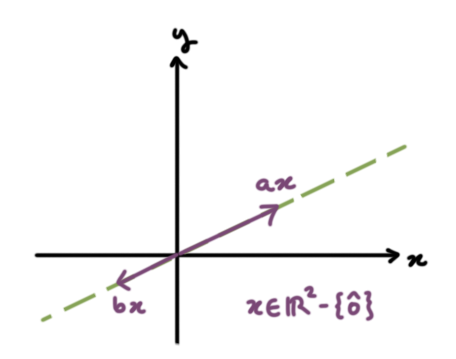
\includegraphics[scale= 2]{27} 
	\caption{Ilustración del primer punto de la Proposición
	\ref{prop: cancelacion en espacio vect} para el caso $V = \IR^{2}$.}
\end{marginfigure}

\begin{itemize}
	\item Sea $x$ un vector no cero, y supongamos que existen escalares $a, b$ distintos
	entre sí tales que $ax = bx$. Entonces, si $c := a - b \neq 0$,
	\[
	c x = (a-b) x = ax - bx = \hat{0}.
	\]
	Como $c$ es un elemento no cero del campo $F$, tiene inverso multiplicativo $c^{-1}$.
	Así,
	\[
	x = 1_{F} \cdot x = (c^{-1} c) \cdot x = c^{-1} \cdot (c \cdot x) = c^{-1} \cdot
	\hat{0} = \hat{0}, 
	\]
	contradiciendo la hipótesis.
	\item \hlgray{Ejercicio}.
\end{itemize}

\QEDB
\vspace{0.2cm}

La versión de la Proposición \ref{prop: cancelacion en espacio vect}
para el $\IR-$espacio vectorial $\IR^{2}$ sería
\begin{center}
	Si $x = (x_{1}, x_{2}) \in \IR^{2}- \{ (0, 0) \}$ y $a, b \in \IR$
	tales que $ax = bx$, entonces $a = b$.
\end{center}
Podemos demostrar esta afirmación directamente; como $x$ no es el vector cero,
sin pérdida de generalidad $x_{1} \neq 0$. De la hipótesis 
\[
(ax_{1}, ax_{2}) = a x = b x = (bx_{1}, bx_{2}) 
\]
se tiene la igualdad en $\IR$ $ax_{1} = bx_{1}$. Como $x_{1} \neq 0$, existe su 
inverso multiplicativo; multiplicando por este a ambos lados de la igualdad, 
se llega a que $a = b$, como se quería.


Nota que la diferencia entre este argumento y el de la demostración de la
Proposición \ref{prop: cancelacion en espacio vect} es que este primero hace
referencia a la forma de los elementos del espacio vectorial $\IR^{2}$, mientras
que el segundo sólo usa los axiomas de campo y espacio vectorial. 

\begin{ejem}
	\textbf{El espacio vectorial trivial:} considere al grupo abeliano $V = \{ 0 \}$ - con 
	la suma definida de la única forma posible. Sea $F$ un campo cualquiera. La
	\textit{única} forma de definir una función $\cdot : F \times V \longrightarrow V$
	es por
	\[
	\forall a \in F: \hspace{0.2cm} a \cdot 0 = 0.
	\]
	Puede comprobar que, con este producto escalar, $V$ es un $F-$ espacio vectorial, 
	al que solemos denominar el \textbf{espacio vectorial cero} o el 
	\textbf{espacio trivial}.
\end{ejem}

\section{Subespacios vectoriales}
En muchas ocasiones, dado $V$ un $F-$espacio vectorial, nos interesará trabajar
con subestructuras de $V$ que ``con la misma suma y multiplicación por escalares'', 
sean en sí mismas espacios vectoriales.

\marginnote{Si $f: A \longrightarrow B$ es una función y $C$ es un subconjunto de 
$A$, por $f_{|C}$ denotamos a la \textbf{restricción de $f$ a $C$}.}
\begin{defi}
		\label{def: de subespacio}
	Sea $(V, +, 0_{V}, F, \cdot : F \times V \longrightarrow V)$ un espacio vectorial.
	Un subconjunto no vacío $\emptyset \neq W \subseteq V$ es un
	\textbf{subespacio vectorial} de $V$ si 
	$$(W, +_{| W \times W}, 0_{V}, F, \cdot_{|F \times W}: F \times W \longrightarrow W)$$
	es un espacio vectorial.
	En este caso, escribimos $W \leq V$.
\end{defi}
En la definición de subespacio, nótese que se está suponiendo que
las restricciones $+_{W \times W}$ y $\cdot_{F \times W}$ 
tengan ambas como codominio a $W$ - pues se están usando para dotar a $W$ 
de estructura de espacio vectorial.

Si quisieramos usar la Definición
\ref{def: de subespacio} para ver si un subconjunto $W$ de
$V$ es subespacio, nota que las propiedades 
$EV5 - EV8$ se cumplen todas ``por herencia de $V$'' - si son ciertas
para todo elemento de $V$, por supuesto que lo son para todo elemento del
subconjunto $W$ de $V$. Entonces, $W$ es subespacio de $V$ si y sólo si  
los codominios de $+_{W \times W}$ y $\cdot_{F \times W}$ son $W$ y 
$(W, +_{W \times W})$ es un grupo abeliano, es decir, si 

\begin{itemize}
	\item Para cualesquiera $x, y \in W$: $x + y \in W$
	\item Para cualesquiera $x \in W$, $a \in F$: $ax \in W$
	\item $0_{V} \in W$
	\item Para todo $x \in W$, también $-x \in W$.
\end{itemize}
De hecho, el cumplir estas
primeras tres condiciones
es necesario y suficiente para ser subespacio.

\begin{teo}
	\label{teo: caracterizacion de subespacios}
	Sea $V$ un $F-$espacio vectorial, $W$ un subconjunto de $V$. 
	Entonces, $W$ es subespacio de $V$ si y sólo si 
	\begin{itemize}
		\item $\hat{0} \in W$
		\item \textit{(Cerradura bajo la suma)} Para cualesquiera $x, y \in W$: $x + y \in W$
		\item \textit{(Cerradura bajo multiplicación escalar)} Para cualesquiera 
		$x \in W$, $a \in F$: $ax \in W$
	\end{itemize}
\end{teo}
\marginnote{El Teorema \ref{teo: caracterizacion de subespacios} es el que en 
la práctica se usa para determinar si $\emptyset \neq W \subseteq V$ es subespacio o no.}
\textbf{Demostración.}
\begin{itemize}
	\item[$\Rightarrow$)] Trivial
	\item[$\Leftarrow$] Por la discusión de arriba, basta ver que, para todo
	$x \in W$, también $-x \in W$, pero esto por la cerradura bajo multiplicación 
	por escalares y la Proposición 
	\ref{prop: hechos basicos ev} se cumple, pues
	\[
	-x = (-1_{F}) \cdot x \in W.
	\]
\end{itemize}
\QEDB
\vspace{0.2cm}

\begin{ejem}
	Dados $a < b$ números reales, 
	considere al $\IR-$espacio vectorial de funciones $\IR^{[a, b]}$. 
	Sea
	\[
	\mathcal{C}(a, b) := \{ f \in \IR^{[a, b]} : \hspace{0.2cm} f \textit{
	es continua en } [a, b] \}.
	\]
	Se demuestra que
	\begin{itemize}
		\item la función constante cero $\hat{0}_{[a, b]}$ es una función continua,
		\item la suma de funciones continuas es continua, y
		\item la multiplicación de una función continua por un escalar resulta en una
		función continua,
	\end{itemize}
	luego, $\mathcal{C}(a, b)$ es un subespacio de $\IR^{[a, b]}$.
\end{ejem}

Muchas veces, si se quiere probar que $W$ es espacio vectorial, resulta más sencillo
verlo como subconjunto de un espacio vectorial y mostrar que es subespacio de este,
pues lo primero requiere comprobar tres condiciones 
(c.f. Teorema \ref{teo: caracterizacion de subespacios}), mientras que lo segundo 
requiere comprobar ocho condiciones 
(c.f. Definición \ref{defi: espacio vectorial}).

\hlgray{Ejercicio:}
	considere al conjunto 
	\[
	U = \{ (x, x, 0, y) \in \IR^{4} : \hspace{0.2cm} x, y \in \IR  \}.
	\]
	Si la suma y multiplicación por escalares se definen entrada a entrada,
	demuestre que $U$ es un $\IR-$espacio vectorial.

\hlgray{Ejercicio:}
sea ahora
\[
U' = \{ (x, x, 1, y) \in \IR^{4} : \hspace{0.2cm} x, y \in \IR  \}.
\]
¿Es $U'$ subespacio de $\IR^{4}$?


\section{El subespacio generado por un subconjunto y suma de subespacios}


Dado $V$ un $F-$espacio vectorial, 
sea $\{ W_{\alpha} \}_{\alpha \in I}$ una familia no vacía de subespacios
de $V$. A partir de esta familia, ¿cómo podemos construir otro
subespacio de $V$?
Consideremos a la unión e intersección de la familia, o sea,
a los conjuntos

\begin{equation}
	\label{eq: int fam subesp}
	\bigcap_{\alpha \in I} W_{\alpha} :=
\{ x \in V  | \hspace{0.2cm} x \in W_{\alpha} \textit{ para toda }
\alpha \in I  \} \subseteq V,
\end{equation}
y
\begin{equation}
	\label{eq: union fam subesp}
	\bigcup_{\alpha \in I} W_{\alpha} :=
\{ x \in V  | \hspace{0.2cm} x \in W_{\alpha} \textit{ para algúna }
\alpha \in I  \} \subseteq V.
\end{equation}

¿Son estos subespacios de $V$?
Tenemos una
respuesta afirmativa y otra negativa.

\begin{prop}
La intersección \eqref{eq: int fam subesp} de la familia
de subespacios $\{ W_{\alpha} \}_{\alpha \in I}$
de $V$ es un subespacio de $V$.
\end{prop}
\noindent
\textbf{Demostración.}
\begin{itemize}
	\item[i)] Puesto que el cero es elemento de \textit{todo}
	subespacio de $V$, claro que $0 \in W_{\alpha}$ para
	toda $\alpha \in I$, luego, $0 \in \bigcap_{\alpha \in I} W_{\alpha}$
	\item[ii, iii)] Sean $x, y \in \bigcap_{\alpha \in I} W_{\alpha}$,
	$a \in F$; claro que 
	$x+y, ax \in \bigcap_{\alpha \in I} W_{\alpha}$
	pues, dado $\alpha \in I$ un índice cualquiera,
	$x, y \in W_{\alpha}$, luego, como 
	$W_{\alpha}$ es subespacio de $V$, $x+y, ax \in W_{\alpha}$.
\end{itemize}

\QEDB
\vspace{0.2cm}

La demostración anterior fue muy sencilla pues, para
que un vector sea elemento de la intersección
$\bigcap_{\alpha \in I} W_{\alpha}$,
debe estar en \textit{todos} los elementos de la familia a la 
vez, y todos los $W_{\alpha}$ cumplen  
los tres puntos de la proposición (*-sub).
La condición que debe cumplir un vector para estár en la 
unión de la familia es mucho más laxa; es necesario y suficiente
que sea elemento de un solo miembro de la familia
$\{ W_{\alpha} \}_{\alpha \in I}$.
Dados
$x, y \in \bigcup_{\alpha \in I} W_{\alpha}$,
existen $\alpha_{1}, \alpha_{2} \in I$
tales que $x \in W_{\alpha_{1}}$ y 
$y \in W_{\alpha_{2}}$. Nota que \textit{no podemos
decir que $x$ y $y$ son elementos de un mismo subespacio}, luego,
esta información no parece implicar que la suma sea elemento de la 
unión.


\begin{ejem}
	\label{ej: subespacios funciones, dominio abierto}
(Que muestra que la unión de subespacios puede no ser un subespacio).
Sea $(a, b) \subseteq \IR$ un intervalo abierto cualquiera.
Considere al $\IR-$espacio vectorial
\[
\IR^{(a, b)} = \{ f: (a, b) \longrightarrow
\IR  | \hspace{0.2cm} f \textit{ es función.} \}
\]

Sean 
\[
\mathcal{B}_{(a, b)} = \{ f \in \IR^{(a, b)}  | \hspace{0.2cm}
f \textit{ es acotada}  \}, \hspace{0.4cm}
\mathcal{C}_{(a, b)} = \{ f \in \IR^{(a, b)}  | \hspace{0.2cm}
f \textit{ es continua}  \}.
\]
Como sabes por tus cursos de cálculo, estos son subespacios
de $\IR^{(a, b)}$. Claro que ninguno de ellos está contenido en el otro
(hay funciones definidas en $(a, b)$ que son continuas pero no acotadas, así
como acotadas pero no continuas).
Nota que 
\begin{itemize}
	\item $\hat{0} \in \mathcal{B}_{(a, b)} \cup \mathcal{C}_{(a, b)}$, y que
	\item si $\lambda \in \IR$ y $f \in \mathcal{B}_{(a, b)} \cup \mathcal{C}_{(a, b)}$,
	entonces también $\lambda f \in \mathcal{B}_{(a, b)} \cup \mathcal{C}_{(a, b)}$,
\end{itemize}
sin embargo, $\mathcal{B}_{(a, b)} \cup \mathcal{C}_{(a, b)}$ \textbf{no} es un
subespacio de $\IR^{(a, b)}$, pues no es cerrado bajo la suma.
En la imagen se muestran la gráfica
de una función continua $f$ y una acotada
$g$ en $(a, b)$ para las que la suma no es ni continua ni 
acotada (i.e. tales que $f, g \in \mathcal{B}_{a, b} \cup
\mathcal{C}_{a, b}$ pero $f + g \not\in \mathcal{B}_{a, b}
\cup \mathcal{C}_{a, b}$). 
\begin{figure}[H]
	\sidecaption{
	Con el sumando continuo rompemos la acotación, y con
el sumando acotado, la continuidad.
	\label{fig: 2}
	}
	\centering
	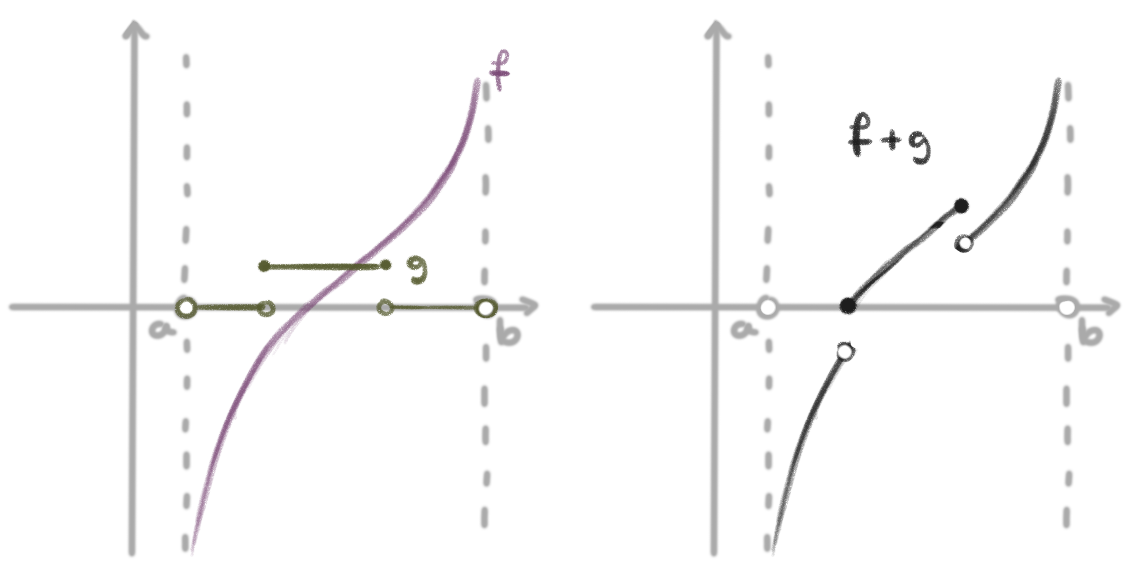
\includegraphics[scale = 2.5]{2} 
\end{figure}	
\diam
\end{ejem}

\begin{ejem}
	\label{ej: subespacios funciones, dominio compacto}
	Ahora considera a los espacios de funciones 
	$\IR^{[a, b]}$, $\mathcal{B}_{[a, b]}$, $\mathcal{C}_{[a, b]}$.
	Demostraste en tu curso de cálculo de una variable que toda
	función con dominio \textbf{cerrado y acotado} que sea continua,
	es también acotada (c.f. \TODO{cita Spivak, p. 178}). Entonces, 
	\[
	\mathcal{C}_{[a, b]} \subseteq \mathcal{B}_{[a, b]},
	\]
	luego, la unión
	\marginnote{Los Ejemplos \ref{ej: subespacios funciones, dominio abierto} y 
	\ref{ej: subespacios funciones, dominio compacto} nos hacen ver que aspectos
	propios del dominio $X$ común a las funciones que conforman el espacio vectorial
	(en particular, su topología), afectan la forma que tengan estos espacios.}
	\[
	\mathcal{C}_{[a, b]} \cup \mathcal{B}_{[a, b]} = \mathcal{B}_{[a, b]}
	\]
	trivialmente es un subespacio de $\IR^{[a, b]}$.
\end{ejem}

\hlgray{Ejercicio:} Si $\{ W_{\alpha} \}_{\alpha \in I}$
es una colección de subespacios de $V$ tal que
\[
(\forall i, j \in I)(\exists k \in I): \hspace{0.2cm}
W_{i}, W_{j} \subseteq W_{k},
\]
entonces $\bigcup_{\alpha \in I} W_{\alpha}$ es un subespacio de $V$.


 \begin{center}
 --- * * * ---
 \end{center}
Ahora, dado $V$ un $F-$espacio vectorial, a veces nos interesará
limitarnos a trabajar no con todo el espacio $V$, sino con un 
subconjunto $X$ de este. Como también queremos aprovechar
la estructura algebráica, nos interesará que tal colección $X$
sea, más que subconjunto, subespacio de $V$.
Esto puede ocurrir o no: lo que siempre podemos hacer
es considerar a la familia $\{ W \leq V : 
\hspace{0.2cm} X \subseteq W \}$ de subespacios más pequeños
(en el sentido que están propiamente contenidos en $V$)
que contienen a nuestro conjunto de interés de $X$, y 
``condensar'' a esta familia via su intersección.

\begin{defi}
Sean $V$ un $F-$espacio vectorial, $X \subseteq V$. 
El subespacio
\begin{equation}
	\label{eq: sub generado por X}
	span (X) := \bigcap \{ W \leq V : \hspace{0.2cm}
	X \subseteq W \},
\end{equation}
o sea, la intersección de la familia de todos los subespacios
de $V$ que contienen a $X$, es llamado el 
\textbf{subespacio de $V$ generado por $X$}.
\end{defi}

\begin{prop}
$span (X)$ es el menor subespacio de $V$
que contiene a $X$, es decir,
\marginnote{Estamos considerando a la contención de conjuntos
como orden; el que un conjunto $A$ sea menor que un conjunto
$B$ significa que $A$ está contenido en $B$.}
\[
\forall \hspace{0.1cm} W \leq V: \hspace{0.2cm}
X \subseteq W \Rightarrow span (X) \leq W.
\]
\end{prop}
\noindent
\textbf{Demostración.}
Es clara pues, $span (X)$, al ser por definición
la intersección de la familia de subespacios que
contienen a $X$, está contenido en cada uno de sus integrantes.

\QEDB
\vspace{0.2cm}

En resumen: si $X$ no es subespacio, siempre podemos
considerar a $span (X)$, \textit{el menor}
subespacio de $V$ que contiene al conjunto de interés.

\hlgray{Ejercicio:} Demuestre que, si $X \leq V$,
entonces $X = span (X)$.

\begin{obs}
Por definición,
$span (\emptyset)$ es la intersección 
de la familia de subespacios que contienen a 
$\emptyset$ - o sea, es la intersección de todos los subespacios
de $V$. Como $\{ 0 \}$ es el menor subespacio de $V$, concluimos que
\[
span (\emptyset)= \{ 0 \}.
\] 
\end{obs}

En \eqref{eq: sub generado por X} decimos cómo
construir teóricamente a tal $span (X)$; el objetivo ahora es dar
una descripción completa de sus elementos, es decir,
dar un criterio concreto en base al cual determinar
cuándo un vector $x$ del espacio pertenece a 
$span (X)$.

Según el Teorema \ref{teo: caracterizacion de subespacios}, 
$X$ puede no ser subespacio
por cumplirse al menos una de las tres razones siguientes:
\begin{itemize}
	\item $\hat{0} \not\in X$; corregimos esto agregando
	al vector cero.
	\item Existen $x, y \in X$ tales que 
	$x+y \not\in X$; esto se puede arreglar agregando
	sumas de elementos de $X$.
	\item Existen $a \in F$ y $x \in X$ para los que
	$ax \not\in X$. Para que esto no ocurra, podemos 
	agregar los múltiplos escalares de los elementos de $X$.
\end{itemize}

Parece que el problema de no ser subespacio se arregla
si agregamos sumas finitas de múltiplos escalares de elementos
de $X$ (pues así estamos forzando a que los tres puntos del
Teorema \ref{teo: caracterizacion de subespacios}
ocurran). Demos un nombre a tales
sumas de elementos de $X$.

\begin{defi}
Sea $V$ un $F-$espacio vectorial, $X \subseteq V$. Una 
\textbf{combinación lineal} en $V$ de elementos de $X$ es cualquier
vector de la forma
\[
\sum_{i=1}^{n} a_{i}x_{i},
\hspace{0.2cm} \textit{ con }
n \geq 1 \textit{ entero, }
x_{i} \in X, a_{i} \in F
\textit{ para toda } 1 \leq i \leq n.
\] 
\end{defi}

Según la discusión anterior, parece que para ``extender''
a $X$ a un subespacio de la forma mínima, hay que agregar
todas las combinaciones lineales de elementos de $X$, pues con esto
parece quedar asegurada la cerradura bajo suma y multiplicación
por escalares. Confirmamos nuestras sospechas con el siguiente resultado.

\begin{prop}
	\label{prop: caract elementos del subesp generado por X}
Si $\emptyset \neq X \subseteq V$, entonces
$span (X)$ consta de todas las combinaciones lineales
de elementos de $X$, es decir,
\begin{equation}
	\label{eq: elementos del generado de X}
span (X) = \left\{ \sum_{i=1}^{n} a_{i}x_{i} | \hspace{0.2cm} 
n \in \IN, x_{i} \in X, a_{i} \in F \hspace{0.2cm} \textit{ para toda }
1 \leq i \leq n \right\}
\end{equation}
\end{prop}
\noindent
\textbf{Demostración.}
Sea 
\[
\mathcal{A} = \left\{ \sum_{i=1}^{n} a_{i}x_{i} | \hspace{0.2cm} 
n \in \IN, x_{i} \in X, a_{i} \in F \hspace{0.2cm} \textit{ para toda }
1 \leq i \leq n \right\};
\]
veamos que $\mathcal{A} = \langle X \rangle$.
\begin{itemize}
	\item[$\supseteq$]] Claro que $\mathcal{A}$ es subespacio de 
	$V$ (\hlgray{Ejercicio:} compruebe los detalles!). Además, 
	$\mathcal{A}$ contiene a $X$ (pues $x = \sum_{i=1}^{1}1_{F} x \in \mathcal{A}$).
	De esto se deduce que $span ( X )\subseteq \mathcal{A}$.
	
	
	\item[$\subseteq$]] Sea ahora
	$a_{1} x_{1} + \ldots + a_{n} x_{n}$ un elemento genérico 
	de $\mathcal{A}$; mostremos que este es elemento de 
	\textit{cualquier} subespacio $W$ de $V$ que contenga a 
	$X$ - de esto podremos concluir la contención deseada, 
	pues $span ( X )$ \textit{es} la intersección 
	de tales subespacios $W$.
	Sea pues $W \leq V$ con $X \subseteq W$. Como cada
	$x_{i}$ es elemento de $X$, todos serán elementos de 
	$W$, luego, como $W$ es subespacio de $V$, es cerrado bajo 
	multiplicaciones escalares y sumas, por lo tanto,  
	$a_{1} x_{1} + \ldots + a_{n} x_{n} \in W$.
\end{itemize}

\QEDB
\vspace{0.2cm}

\begin{defi}
Si $\{ W_{\alpha} \}_{\alpha \in I}$ es una familia de subespacios
de $V$, definimos a su suma como el subespacio generado por su unión,
es decir,
\begin{align}
	\label{eq: suma de subespacios}
\sum_{\alpha \in I} W_{\alpha} := &
span \left( \bigcup_{\alpha \in I} W_{\alpha} 
\right) \nonumber \\
= & \left\{ a_{1}w_{1} + \cdots +
a_{n}w_{n}  | \hspace{0.2cm} n \geq 1, a_{i} \in F,
w_{i} \in \bigcup_{\alpha \in I} W_{\alpha} \right\} \nonumber \\
= & \{ a_{1}w_{1} + \ldots + 
a_{n}w_{n}  | \hspace{0.2cm} n \geq 1,
a_{i} \in F, w_{i} \in W_{\alpha} 
\hspace{0.1cm} \textit{ para alguna } \alpha \in I \}.
\end{align}
\end{defi}

\hlgray{Ejercicio:} Demuestre que una forma equivalente de
escribir al subespacio \eqref{eq: suma de subespacios}
es como
\begin{equation}
	\label{eq: suma de subespacios simplificado}
	\sum_{\alpha \in I} W_{\alpha} =
	\{ w_{1} + \cdots + w_{n} : \hspace{0.2cm}
	n \geq 1, w_{i} \in W_{i} \hspace{0.1cm} \forall 1 \leq i \leq n  \}.
\end{equation}


Recapitulemos: dados $W_{1}, W_{2} \leq V$,
\begin{itemize}
	\item $W_{1} \cap W_{2}$ es un subespacio de $V$,
	\item $W_{1} \cup W_{2}$ es subespacio si y sólo si 
	$W_{1} \subseteq W_{2}$ o bien $W_{2} \subseteq W_{1}$. Nota
	que el resultado de esta operación no da lugar a un nuevo
	subespacio de $V$.
	\item El menor subespacio de $V$ que contiene a $W_{1}$
	y $W_{2}$ es su suma, o sea, 
	\[
	W_{1} + W_{2} = \{ w_{1} + w_{2}  | \hspace{0.2cm} 
	w_{1} \in W_{1}, w_{2} \in W_{2} \}.
	\]
\end{itemize}

\begin{defi}
Si $X \subseteq V$ es tal que $span(X) = V$,
decimos que \textbf{$X$ genera al espacio $V$}.
\end{defi}
Es decir, $X$ genera a a $V$ si no hay subespacios propios
de $V$ que contengan a $X$; esto, según la proposición
\ref{prop: caract elementos del subesp generado por X}, significa que
\textit{todo elemento de $V$ puede expresarse como combinación
lineal finita de elementos de $X$}.

\subsection{Suma directa de subespacios}

Sean $V$ un $F$-espacio vectorial, 
$\{ W_{i} \}_{i=1}^{n}$ una familia finita de subespacios
de $V$. Por la proposición 
\ref{prop: caract elementos del subesp generado por X}
sabemos que \textit{todo} elemento de 
su suma es de la forma 
$w_{1} + \ldots + w_{n}$, con $W_{i} \in W_{i}$ para
$1 \leq i \leq n$.

\begin{ejem}
Sea el $\IR-$espacio vectorial $\IR^{3}$. Considere a los subespacios
\[
W_{1} = \{ (a, b, 0)  | \hspace{0.2cm} a, b \in \IR \}
\leq \IR^{3},
\]
\[
W_{2} = \{ (0, c, d)  | \hspace{0.2cm} c, d \in \IR \}
\leq \IR^{3}.
\]
Es claro que $\IR^{3} = W_{1} + W_{2}$; de hecho, dado
$(x, y, z) \in \IR^{3}$ un vector cualquiera del espacio, 
para toda $\alpha \in \IR$ se tiene que
\marginnote{Las entradas cero de los elementos de $W_{1}$
y $W_{2}$ determinan las entradas $x$ y $z$ en la ecuación
\eqref{eq: 1, 21 Ag}, 
pero en las entradas centrales tenemos libertad de elección
-esto se ve reflejado por el parámetro $\alpha$.}
\begin{equation}
	\label{eq: 1, 21 Ag}
	(x, y, z) = (x, \alpha y, 0) + 
(0, (1-\alpha)y, z).
\end{equation}

Esto muestra que hay \textit{una infinidad} de formas
de expresar a un 
vector $(x, y, z) \in \IR^{3}$ como suma
de elementos de $W_{1} \cup W_{2}$.

Considere ahora a los subespacios
\[
V_{1} = \{ (a, 0, 0)  | \hspace{0.2cm} a\in \IR \},
\]
\[
V_{2} = \{ (0, b, 0)  | \hspace{0.2cm} b\in \IR \},
\]
\[
V_{1} = \{ (0, 0, c)  | \hspace{0.2cm} c\in \IR \}.
\]
Claro que $\IR^{3} = V_{1} + V_{2} + V_{3}$; dado
$(x, y, z) \in \IR^{3}$ cualquiera,
\[
(x, y, z) = (x, 0, 0) + (0, y, 0) + (0, 0, z).
\]
Una representación de esta forma es única. Por ejemplo,
el que las primeras entradas de los últimos dos sumandos
deban ser cero (por definición de $V_{1}$ y $V_{2}$)
forza que la primera entrada del primer sumando sea $x$.
\diam
\end{ejem}

\begin{defi}
Sea $\{ W_{i} \}_{i=1}^{n}$ una familia finita de subespacios
de $V$. 
\marginnote{El símbolo $\oplus$ es usado para representar
una propiedad del espacio suma $\sum_{i=1}^{n} W_{i}$,
a saber, la unicidad de las representaciones de sus elementos
como sumas de vectores en $\bigcup_{i=1}^{n}W_{i}$.}
El subespacio suma $\sum_{i=1}^{n} W_{i}$
es llamada una \textbf{suma directa} si cada uno de sus
elementos tiene una única representación de la forma
\[
w_{1} + \cdots  + w_{n}, 
\hspace{0.2cm} \textit{ con }
w_{i} \in W_{i}.
\]
En este caso, al subespacio $\sum_{i=1}^{n}W_{i}$
se le denota por
\[
W_{1} \oplus \cdots \oplus W_{n}.
\]
\end{defi}

\begin{prop}
	\label{prop: suma directa sii interseccion cero}
Sean $U, W$ subespacios de $V$. La suma
$U+ W$ es directa si y sólo si $U \cap W = \{ \hat{0} \}$.
\end{prop}
\noindent
\textbf{Demostración.}
\begin{itemize}
	\item[$\Rightarrow$]] Si existe $x \in U \cap W$
	con $x \neq \hat{0}$, entonces, 
	\[
	x = \hat{0} + x, \hspace{0.2cm} \textit{ con }
	\hat{0} \in U, x \in W,
	\]
	y 
	\[
	x = x + \hat{0}, \hspace{0.2cm} \textit{ con }
	x \in U, \hat{0} \in W,
	\]
	luego, la suma $U + W$ no es directa.
	
	\item[$\Leftarrow$]] Sea $x \in U + W$; sean
	$u_{1}, u_{2} \in U$ y $w_{1}, w_{2} \in W$ tales que
	\[
	u_{1} + w_{1} = x = u_{2} + w_{2}.
	\]
	Entonces, 
	\[
	u_{1} - u_{2} = w_{2} - w_{1} \in U \cap W = \{ 0 \},
	\]
	o sea, $u_{1} = u_{2}$ y $w_{1} = w_{2}$.
	
	
\end{itemize}

\QEDB
\vspace{0.2cm}

Note lo siguiente: según el Teorema
\ref{teo: caracterizacion de subespacios},
todos los subespacios tienen en común al 
vector cero $\hat{0}$ del espacio, luego, no tiene sentido
buscar subespacios disjuntos. Lo más disimiles que pueden
llegar a ser $U, W \leq V$ es que su intersección sea
$\{ 0 \}$. Esto, según la Proposición 
\ref{prop: suma directa sii interseccion cero}, 
equivale a que la suma $U + W$ sea directa.


\begin{center}
Suma de subespacios $\sim$ Unión de subconjuntos \\
Suma directa de subespacios 
$\sim$ Unión disjunta de subconjuntos
\end{center}

Note que en la Proposición \ref{prop: suma directa sii interseccion cero}
estamos lidiando sólo con dos subespacios. ¿Podemos generalizar
este resultado para la suma de $n$-subespacios? ¿Será cierto que
la suma $\sum_{i=1}^{n} W_{i}$ es directa si y sólo si 
la intersección $\bigcap_{i = 1}^{n} W_{i}$ es $\{ \hat{0} \}$?
La respuesta es \textbf{no} (c.f. ejercicio
\ref{ej: de la suma directa}). \TODO{Poner la teoría general de suma directa?
La necesito para el tema de diagonalización.}


\section{Caso práctico: Representación de información nutricional}

Veamos cómo los conceptos introducidos pueden ser de utilidad
para modelar y resolver una problemática de la vida real.

Supongamos que a una nutrióloga le interesa
la ingesta de 
\begin{itemize}
	\item calorías
	\item agua
	\item hidratos de carbono 
	\item fibra
	\item grasas, y 
	\item proteinas
\end{itemize}
que un paciente puede obtener al consumir frutas de cierto
grupo de interés (por ejemplo, las frutas que puede encontrar
a precio accesible en su entorno). Sus datos iniciales son
los valores de dichos componentes presentes en las frutas
de interés, datos presentados en forma de tabla como
se muestra a continuación.

\begin{figure}[H]
	\sidecaption{
	Fuente: 
	\url{gruporem-ucam.com}
	\label{fig: tabla frutas}
	}
	\centering
	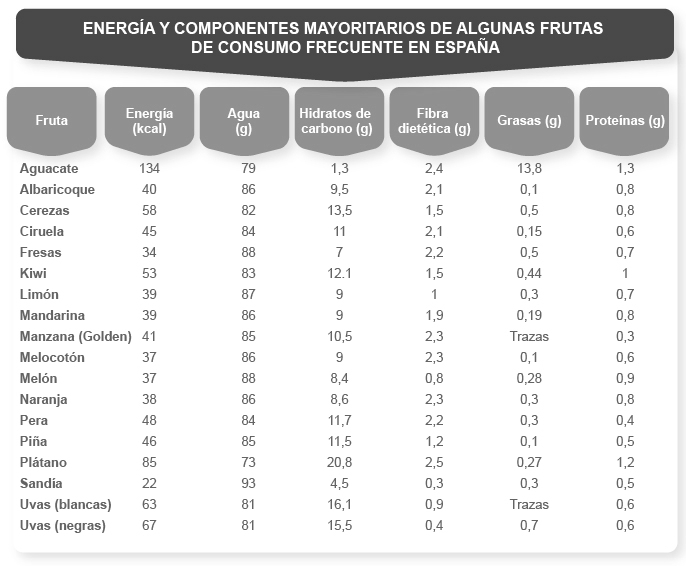
\includegraphics[scale = 0.5]{tablaFrutas} 
\end{figure}	

Algunos de sus pacientes son alérgicos a las frutas de
su lista; digamos que su nuevo paciente no puede 
comer manzanas. La nutrióloga se pregunta si es posible
sustituir los nutrientes aportados por una manzana
con otras frutas de la lista y, si la respuesta es afirmativa,
quisiera dar explícitamente combinaciones de frutas que 
aporten lo mismo que aportaba una cierta cantidad de manzanas
(que no pueden ser incluidas en la dieta del paciente). 
¿Cómo podemos modelar esta situación?

Podemos representar nuestros datos iniciales como
vectores de $\IR^{6}$; por ejemplo, el vector
nutricional de una manzana sería
\[
x_{manzana} = (41, 85, 10.5, 2.3, 0, 0.3)
\in \IR^{6}.
\]
Definamos a $\mathcal{A}$ como el subconjunto de $\IR^{6}$
que consta de todos los vectores fruta,
\[
\mathcal{A} = \{ x_{aguacate}, x_{albaricoque}, \ldots , x_{uvasB},
x_{uvasN} \}.
\]

Nota que, en este contexto, las combinaciones lineales
con coeficientes naturales tienen una interpretación física; por
ejemplo, el vector
\[
2x_{pera} + 5 x_{fresa} + 3 x_{cereza}
\]
representa la información nutrimental de 2 peras,
5 fresas y 3 cerezas (luego, la cantidad de calorías y componentes
que alguien estaría obteniendo al consumir esta cantidad de frutas).

El problema de la nutrióloga queda expresado en términos
de álgebra lineal como sigue:
¿es $x_{manzana}$ elemento del subespacio de $\IR^{6}$ generado
por los vectores $x_{aguacate}, x_{albaricoque}, \ldots ,
x_{uvaB}, x_{uvaN}$? Nota que, implícitamente,
el problema nos permite limitarnos al conjunto de
las combinaciones lineales finitas de los vectores fruta
(menos el vector manzana) y no considerar a todo $\IR^{6}$
(para este problema, no nos interesan vectores que no sean combinaciones
lineales de vectores fruta). La teoría estudiada antes nos asegura que
\begin{itemize}
	\item Tal conjunto de combinaciones de vectores fruta
	es un subespacio de $\IR^{6}$ y,
	\item de hecho, es el menor subespacio de $\IR^{6}$ que contiene 
	a los vectores fruta menos el manzana.
\end{itemize}

La pregunta de la nutrióloga queda entonces expresada en ver si ocurre
\[
x_{manzana} \in span ( \mathcal{A} - \{ x_{manzana} \} )
\]
o no.
\marginnote{No nos interesan todos los elementos de $\IR^{6}$, sino
sólo aquellos que sean combinaciones lineales de vectores fruta;
estamos reemplazando a nuestro espacio de trabajo $\IR^{6}$
por $\langle \mathcal{A} \rangle$.}

Observa que \textbf{los vectores son mucho más que una forma conveniente de 
almacenar información: podemos hacer operaciones de ellos e
interpretarlas en el contexto del 
problema físico planteado}.

Con las definiciones e ideas que planteamos en los siguientes capítulos,
podremos 
\begin{itemize}
	\item determinar cuándo existen combinaciones de frutas
	que aporten lo mismo que cierta cantidad de manzanas,
	\item decir si hay una única forma o varias de expresar manzanas
	en términos de combinaciones lineales de frutas específicas,
	\item usar argumentos de dimensionalidad para determinar
	cuándo subconjuntos de frutas son suficientes para
	sustituir a todas las demás,
\end{itemize}
entre otras cosas.
Es fácil pensar requerimientos razonables
que complicarían aún más la situación; por ejemplo, considera que,
en un escenario realista, 
\begin{itemize}
	\item un paciente podría tener no sólo posibles alergias
	como limitantes para definir una dieta, sino también 
	un presupuesto mensual que no pueda sobrepasar, presupuesto
	que podría reducir aún más las opciones o cantidades
	de fruta que puede consumir (por ejemplo, esto podría implicar
	que combinaciones lineales que contengan al vector
	$x_{aguacate}$ sólo sean consideradas cuando su coeficiente
	-i.e. el escalar por el que se multiplica a $x_{aguacate}$ - 
	no sea mayor a cierto valor).
\end{itemize}



\begin{figure}[H]
\centering\captionsetup{format = hang}
	\begin{measuredfigure}
		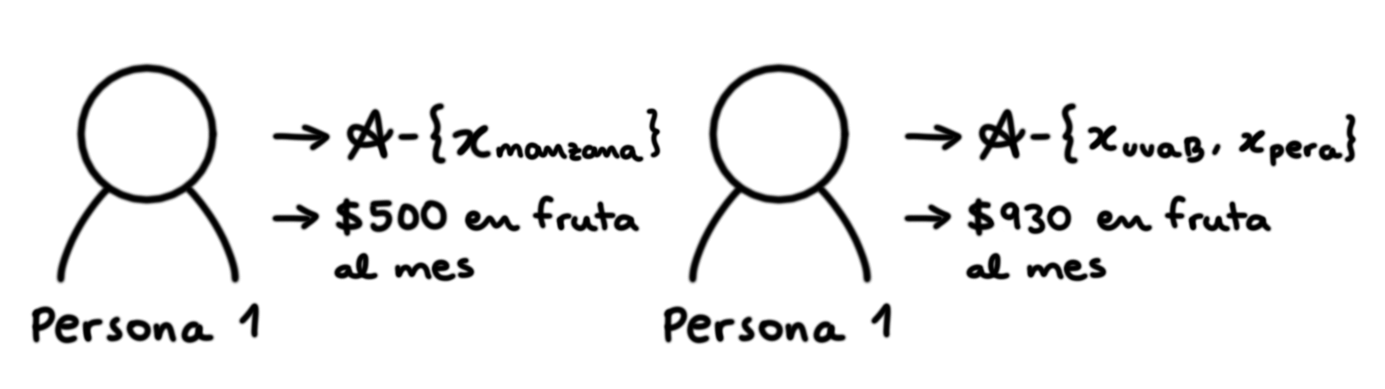
\includegraphics[scale=2]{3} 
		\caption{Cada paciente tiene sus necesidades personales,
		por ejemplo, las frutas a las que es alérgico (o que no le
		gustan, y quiere evitar en su dieta) y su presupuesto mensual.
		Esto cambia el espacio de combinaciones lineales a considerar
		para cada uno, por lo tanto, las combinaciones lineales aceptables
		para construirle una dieta.}
 	\end{measuredfigure}
 \end{figure}

Incluso en esta situación tan simplificada, vemos la utilidad
de usar el marco teórico ofrecido por el álgebra lineal para
modelar la situación; con los conocimientos de los próximos
capítulos seremos capaces de resolver los problemas
aquí planteados. 